\documentclass[11pt,letterpaper]{article}

% Load package
\usepackage{lesson}
\usepackage{amsmath}
\usepackage{xcolor}

%--------------------------------------%
% Custom commands include:             %
%%%%%%%%%%%%%%%%%%%%%%%%%%%%%%%%%%%%%%%%
% Include an image:                    %
% \diagram{height}{align}{file}        %
%                                      %
% height: a number representing mm     %
% align: left, center, or right        %
% file: file name without extension    %
%%%%%%%%%%%%%%%%%%%%%%%%%%%%%%%%%%%%%%%%
% Add a numbered question:             %
% \question{text}                      %
% \questiond[lines]{file}{width}{text} %
%                                      %
% lines: # of lines of text to wrap    %
% file: file name without extension    %
% width: a % of textwidth for image    %
%%%%%%%%%%%%%%%%%%%%%%%%%%%%%%%%%%%%%%%%
% Add a lettered option/question part: %
% \option[vspace]{text}                %
%                                      %
% vspace: added space above the option %
%%%%%%%%%%%%%%%%%%%%%%%%%%%%%%%%%%%%%%%%
% Add a blank line in text:            %
% \blankline{width}                    %
%%%%%%%%%%%%%%%%%%%%%%%%%%%%%%%%%%%%%%%%
% Add an arc symbol in math:           %
% \arc{notation}                       %
%--------------------------------------%
%%%%%%%%%%%%%%%%%%%%%%%%%%%%%%%%%%%%%%%%
%--------------------------------------%
% To reset the question counter:       %
% \setcounter{qcounter}{0}             %
%                                      %
% To reset the option counter:         %
% \setcounter{acounter}{0}             %
%--------------------------------------%

% Set title and course name
\settitle{Week 1 Question Set}
\setsubtitle{Simple neuron model \& Vision: An Overview}
\setcourse{Summer 2023}

\begin{document}

% Create title and add proper header for first page
\maketitle
\thispagestyle{first}

\section{CNS1.1 - Neuron and Synapses} % or Analyze, Experiment, etc.
\begin{enumerate}
    \item Who is widely regarded as the father of modern neuroscience and is also renowned for his detailed drawings of neurons and brain structures? \emph{Hint}: He was from Spain and won a Nobel Prize for this work.
    \vspace{0.5in}
    
    \item Please refer to the figure below, which depicts a drawing of a neuron. Please label the following parts of the drawing with the appropriate names.
    \begin{center}
        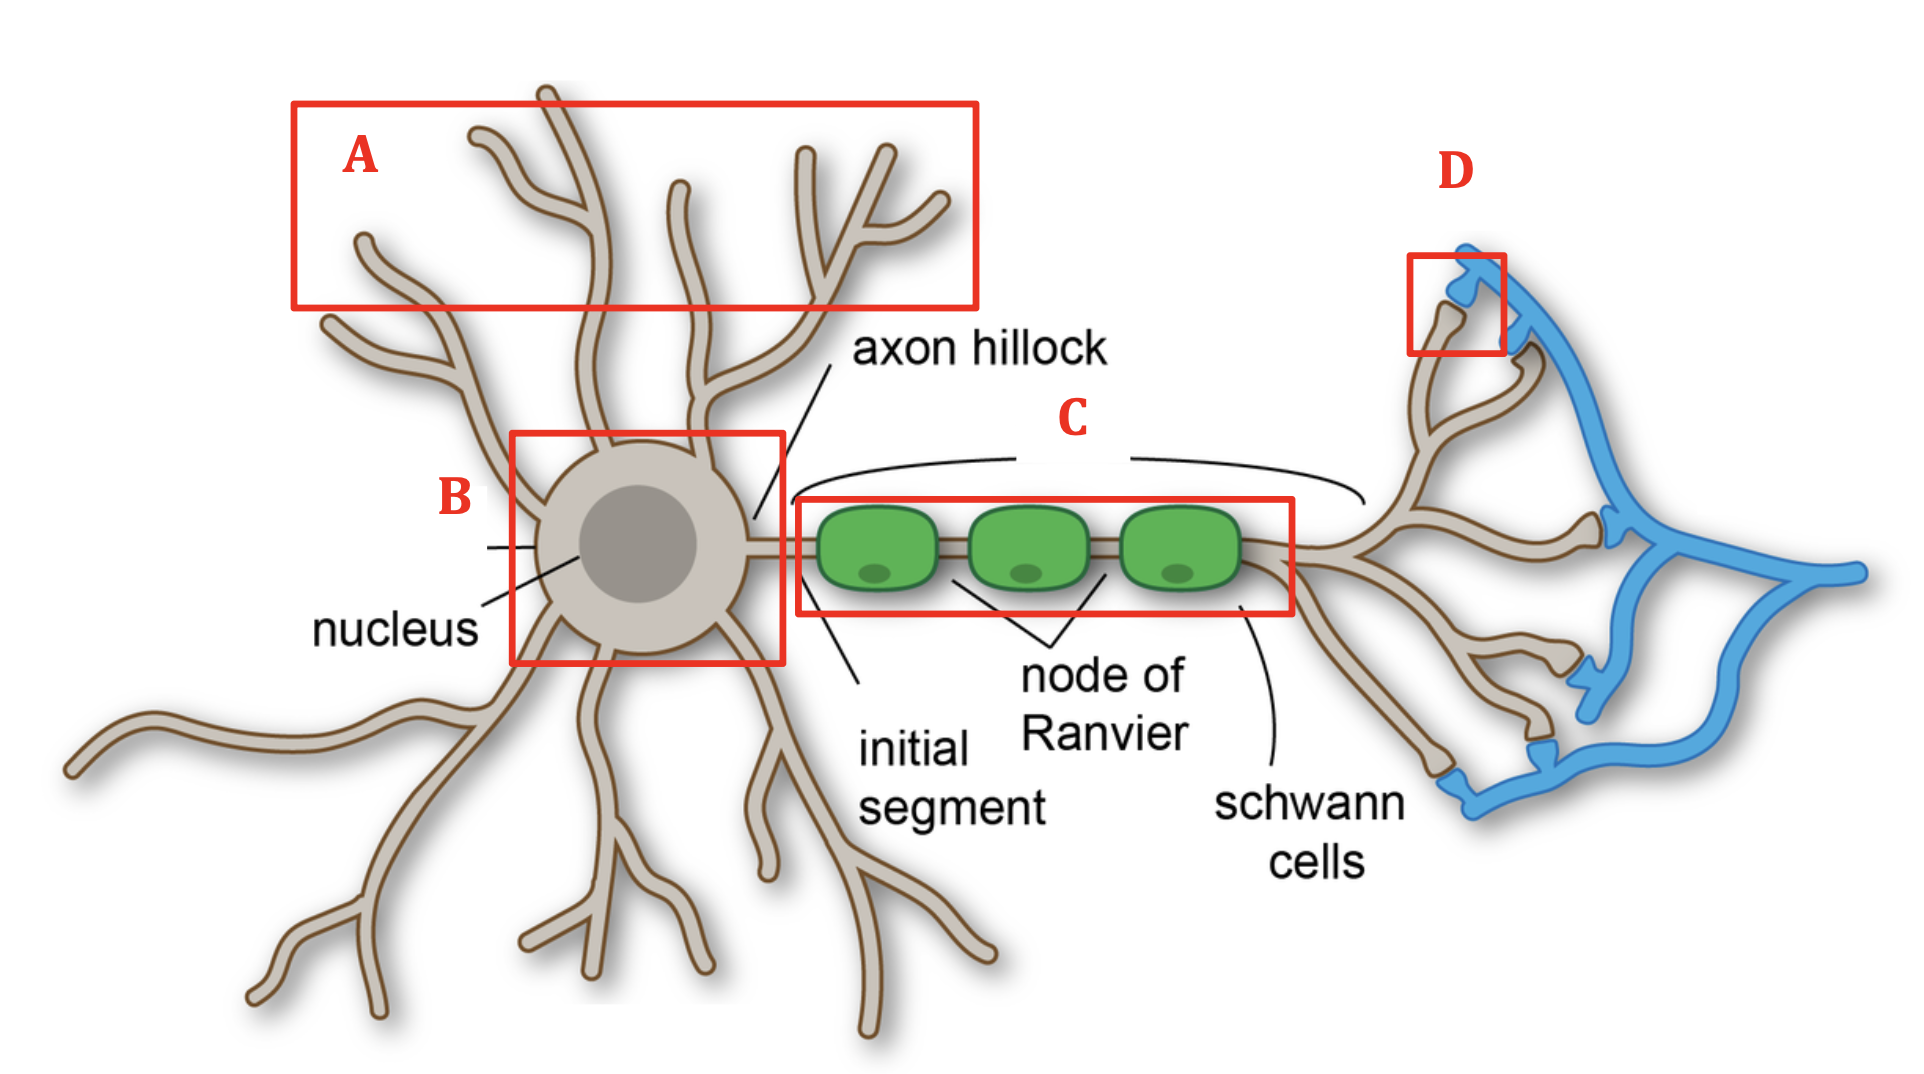
\includegraphics[scale=0.4]{1.2.png}
    \end{center}
    \begin{enumerate}
        \item[A:]
        \item[B:]
        \item[C:]
        \item[D:]
    \end{enumerate}

    \item Circle the appropriate options: It is common to refer to the sending neuron as the (pre/post)synaptic cell and to the receiving neuron as the (pre/post)synaptic cell.
    
\end{enumerate}

\section{CNS1.2 - The Passive Membrane}
\begin{enumerate}
    \item Let's derive the same differential equation for the passive membrane model:
    \begin{align*}
        \tau \cdot \frac{d}{dt} V(t) = - V(t) + R \cdot I(t),
    \end{align*}
    where $\tau = R \cdot C$ is the time constant, $V(t)$ is the membrane voltage, $R$ is the membrane resistance, and $I(t)$ is the current through the membrane.
    \begin{center}
        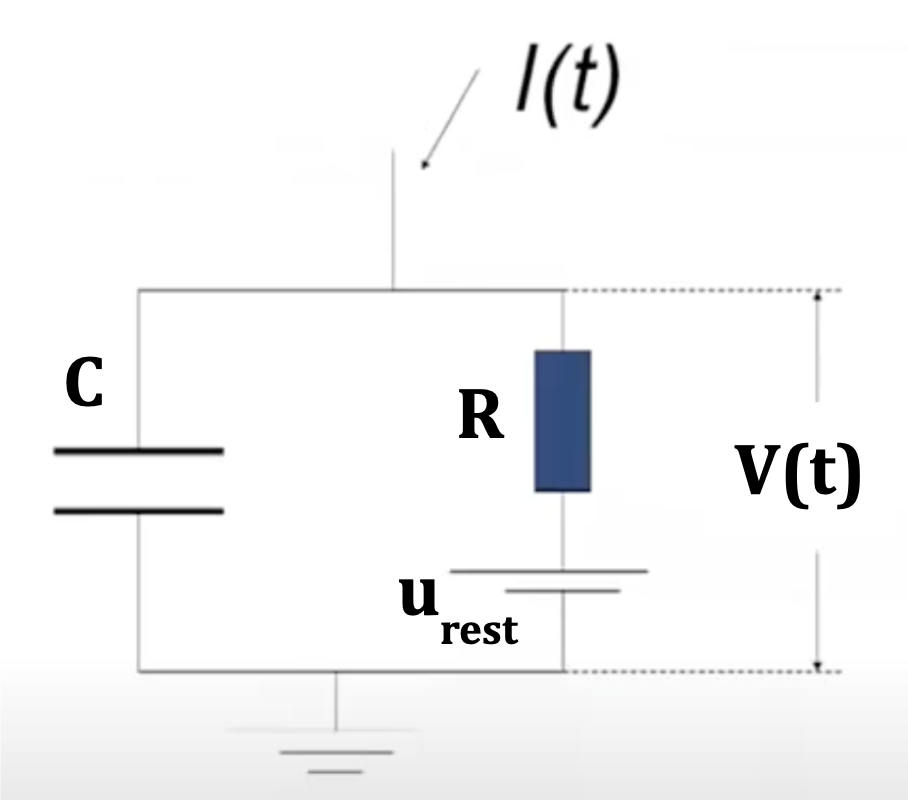
\includegraphics[scale=0.5]{2.1.png}
    \end{center}
    Start off by using Kirchhoff's Current Law: $I(t) = I_C(t) + I_R(t)$. \emph{Hint}: Feel free to use the following well-known differential equations to simplify the steps:
    \begin{align*}
        I_C(t) &= C \frac{d}{dt} V(t)\\
        I_R(t) &= \frac{V(t)}{R}
    \end{align*}
    It is actually a lot easier than what the lecture shows.
    
    
    \pagebreak
    
    \item It is time to interpret the differential equation for the passive membrane model. Circle the most correct option:
    \begin{enumerate}
        \item What causes the membrane to have a capacitance $C$?
        \begin{enumerate}
            \item The concentration gradient of ions.
            \item Its ability to separate opposite charges across a surface.
            \item The speed of action potentials.
            \item Its production of ATP molecules.
        \end{enumerate}
        \item What directly contributes to the electrical resistance $R$ of a biological membrane?
        \begin{enumerate}
            \item The fact that it is made of two instead of one layer of phospholipids.
            \item The finite transportation rate of the ions by membrane proteins and ion channels.
            \item The pH level of the surrounding cellular environment.
        \end{enumerate}
        % \item The membrane voltage $V(t)$, by convention, is defined as:
        % \begin{enumerate}
        %     \item $V_{in} - V_{out}$
        %     \item $V_{out} - V_{in}$
        % \end{enumerate}
        \item What is the significance of the time constant $\tau$?
        \begin{enumerate}
            \item It determines the rate at which a circuit can transfer energy.
            \item It quantifies the amount of resistance present in a circuit.
            \item It characterizes the responsiveness of a circuit to changes in input signals.
            \item It measures the efficiency of power transmission in a circuit.
        \end{enumerate}
        \item What is false about the Dirac delta function?
        \begin{enumerate}
            \item It is denoted by \(\delta\).
            \item It has infinite height and no width.
            \item It has an area under the curve of one, i.e., it integrates to one.
            \item It is a continuous and differentiable function.
        \end{enumerate}
        \item A fictional passive membrane with a resting potential of 0.00 mV has just been charged to 1.00 mV. After 1 $\tau$, what is the expected membrane voltage?
        \begin{enumerate}
            \item 0.63 mV
            \item 1.00 mV
            \item 0.37 mV
            \item 0.50 mV
        \end{enumerate}
    \end{enumerate}
\end{enumerate}
\pagebreak

\section{CNS1.3 - Leaky Integrate-and-Fire Model}
Given the Leaky Integrate-and-Fire (LIF) model:
\begin{align*}
    \tau \cdot \frac{d}{dt} u(t) = - \left( u(t) - u_{rest}\right) + R \cdot I(t),
\end{align*}where $u(t)$ is reset to $u_{rest}$ every time $u(t)$ reaches the threshold $\theta$. Let's assume the input current $I(t)$ is actually constant-valued $I_0$. Find the frequency-current relationship $f = g(I_0)$, i.e., frequency as a function of different levels constant current $I_0$. \emph{Note}: I changed the notation from $V(t)$ to $u(t)$ to be consistent with the video. Also, here I am assuming the neuron is reset back to $u_{rest}$, but the video uses $u_{reset} = u_r$, which may or may not be $u_{rest}$.

\begin{enumerate}
    \item First, let's solve the differential equation to get $u(t)$. Notice that, after some algebraic manipulations, this is a first-order linear differential equation of the form:
    \begin{align*}
        \frac{du}{dt} + p(t)u = g(t)
    \end{align*}
    We can use the mothod of integrating factor. Multiplying the whole equation by the integrating factor $e^{\int p(t) dt}$, we can make the left-hand side become the derivative of a product.
    \vspace{4 cm}
    
    \item Set $u(t) = \theta$ and solve for $t$. This tell us the time it takes for $u$ to reach the threshold $\theta$.
    \vspace{4 cm}

    \item Lastly, take the inverse of the $t$ to get the frequency $f$. You should get a function that is parameterized by $\theta$, $u_{rest}$, $R$, $\tau$, and $I_0$.
\end{enumerate}
\pagebreak

\section{CNS1.4 - Generalized Integrate and Fire Models}
\begin{enumerate}
     \item LIF model can be generalized by replacing the $- \left( u(t) - u_{rest}\right)$ term with a nonlinear function $F(u)$, giving us the Nonlinear Integrate and Fire (eIF) model:
    \begin{align*}
        \tau \cdot \frac{d}{dt} u(t) = F(u) + R \cdot I(t),
    \end{align*}
    Give the names of two common $F(u)$'s?
    \vspace{1 cm}

    \item This video introduces a plot where the x-axis represents the variable $u$, while the y-axis represents the derivative of $du/dt$. Select the wrong statement about this plot:
    \begin{center}
        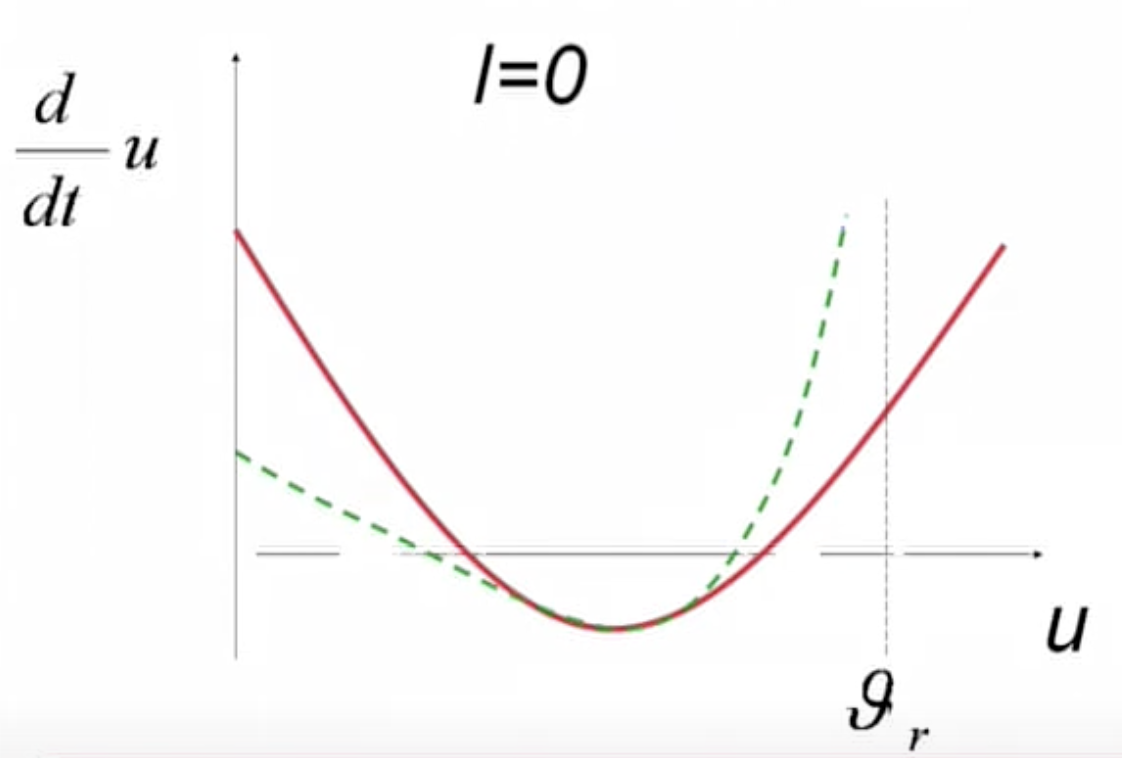
\includegraphics[scale=0.4]{4.1.png}
    \end{center}
    \begin{enumerate}
        \item This plot is known as a phase portrait and phase diagram.
        \item The points where $du/dt = 0$ is known as the fixed point.
        \item The plot can directly determine if the system is linear or nonlinear.
        \item The shape and direction of trajectories provide insights into the behavior of the system.
    \end{enumerate}

    \item Compare between LIF and eIF models: when does repetitive firing happen for each type of the model? 
\end{enumerate}
\pagebreak

\section{V\&B Chapter 1 - Vision: An Overview}
\begin{enumerate}
    \item Given the inherent ambiguity in interpreting 3D objects from stationary 2D retinal images—as exemplified by the wire-frame objects shown in Figure 1.5—what does the author propose as a potential strategy used by the brain to resolve such ambiguities and accurately perceive the 3D structure?
    \vspace{4 cm}
    
    \item The author suggests that our brains have a hierarchy of assumptions when interpreting images, with more critical assumptions overriding less essential ones. An example of this can be seen in the Rubin Vase illusion, a bistable image that our brains can interpret in two distinct ways: as a vase or as two faces in profile. Considering the relative ease with which we can perceive both interpretations, this illusion might represent a case where the two assumptions are of comparable importance. What might this tell us about the hierarchical nature of perceptual assumptions? \emph{Note}: this question is very open-ended.
    \begin{center}
        
\includegraphics[scale=0.1]{rubin.png}
    \end{center}

    \pagebreak

    \item Consider the following descriptions related to a digital calculator and determine which level of Marr's three levels of analysis each corresponds to:
    \begin{enumerate}
    \item[a.] The calculator is used to perform arithmetic computations such as addition, subtraction, multiplication, and division to provide users with a quick, accurate method for performing mathematical calculations.
    \item[b.] The algorithms and representations are implemented physically in the calculator's electronic circuitry, which can involve a range of components including a microprocessor, memory, and input/output devices like buttons and a screen.
    \item[c.] The calculator implements these computations using specific algorithms like the method of successive approximation for calculating square roots. It also uses specific data structures to store and manipulate numbers during computations.
    \end{enumerate}
    Match each description with the correct level of analysis:
    \begin{enumerate}
    \item[i.] Computational Level
    \item[ii.] Algorithmic/Representational Level
    \item[iii.] Physical/Implementation Level
    \end{enumerate}


    
\end{enumerate}




\end{document}